
\begin{figure*}
\vspace{-2ex}
    \centering
    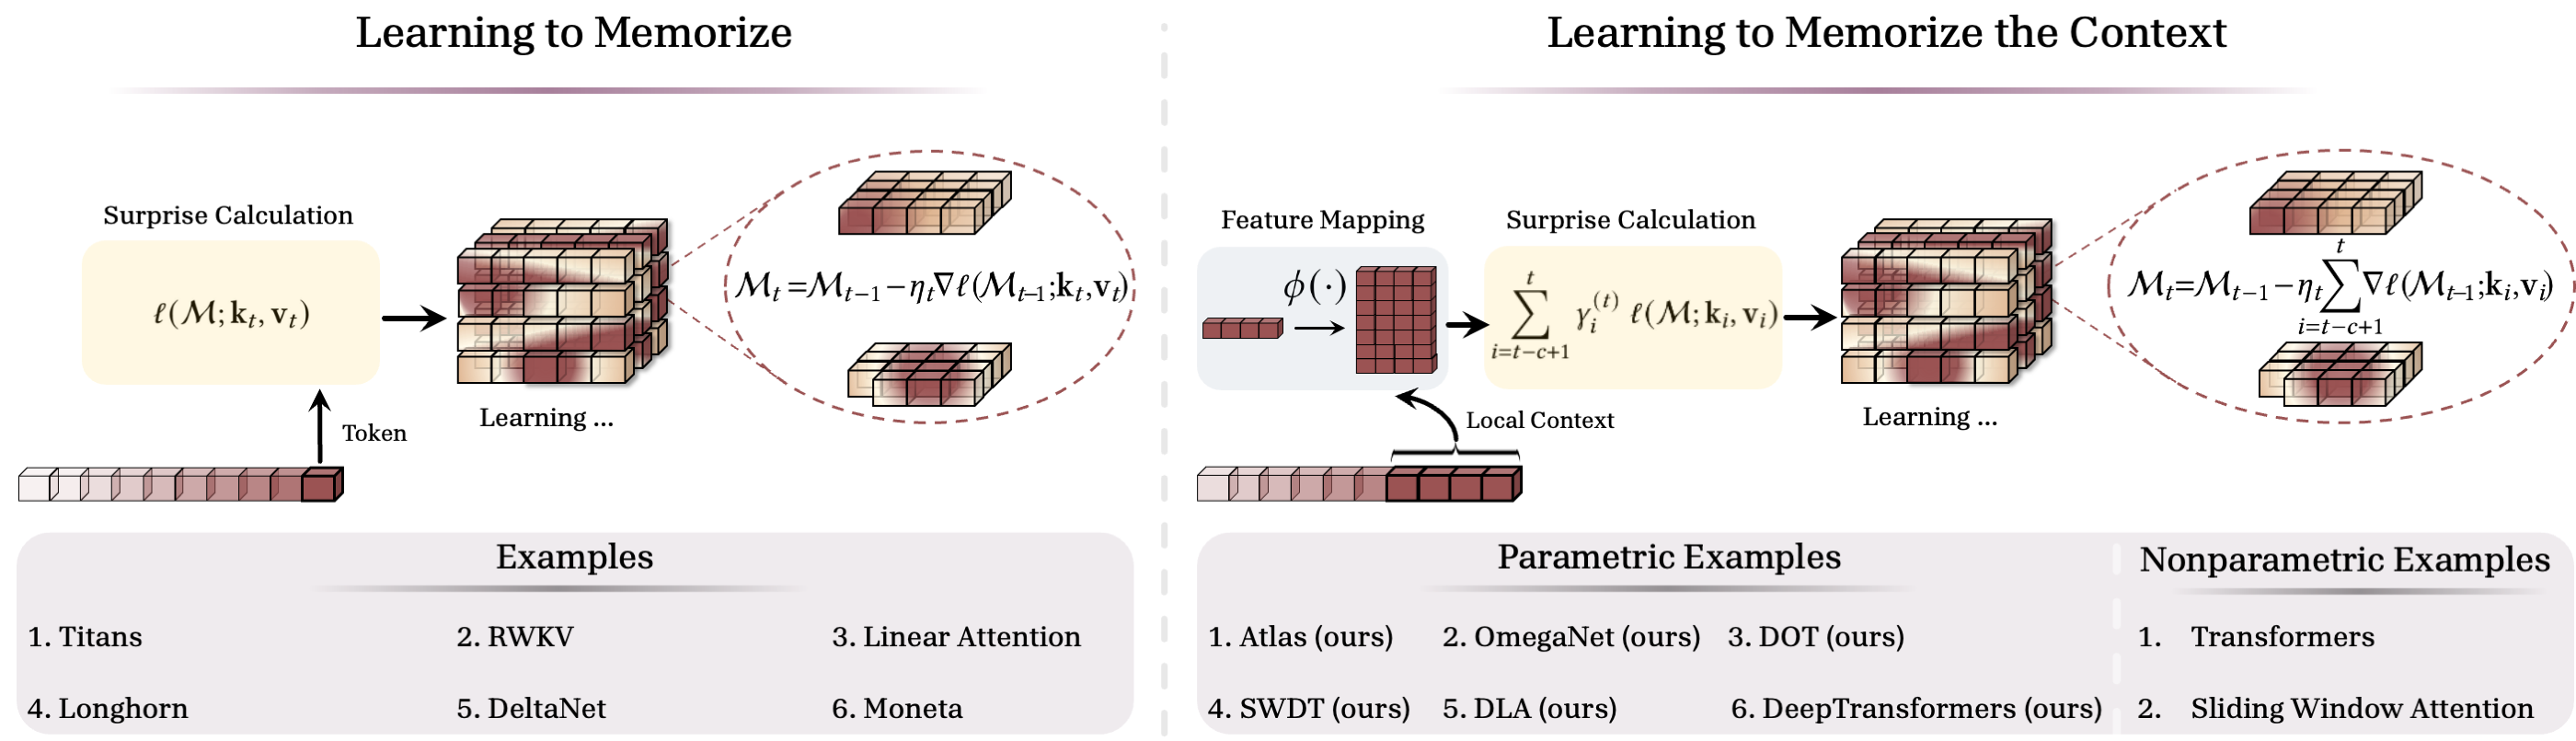
\includegraphics[width=\linewidth]{Images/OmegaRule-Example.png}
    \caption{Comparison of learning to memorize (\textbf{Left}) individual tokens, and (\textbf{Right}) the context.}
    \vspace{-2ex}
    \label{fig:omega-rule-examples}
\end{figure*}


\section{Learning to Memorize the Context at Test Time}
Long-term associative memory, crucial for human learning~\citep{terry2017learning}, has inspired many artificial neural architectures~\citep{he2024camelot, krotov2016dense, LSTM, ramsauer2021hopfield, hopfield1982neural, behrouz2024titans, behrouz2025Miras}. While many such models use matrix- or vector-valued memory to compress past data~\citep{von2023uncovering, yang2024gated, schlag2021linear}, recent studies advocate for deep non-linear neural memory that encodes past abstractions into its parameters~\citep{sun2024learning, behrouz2024titans, behrouz2025Miras, dalal2025one}. For long-context reasoning/understanding, however, these long-term neural memory modules still require: (1) High capacity—the maximum (key, value) pairs storable in parameters (see \textcolor{c1}{\S}\ref{sec:capacity}); (2) A powerful internal memory objective (i.e., \emph{attentional bias}) to learn complex mapping between keys and values (see \textcolor{c1}{\S}\ref{sec:omega-rule}); (3) Powerful memory management for better fixed-size memory management (see \textcolor{c1}{\S}\ref{sec:omega-rule}); and (4) An efficient parallel training process for large-scale training on modern accelerators (see~\textcolor{c1}{\S}\ref{sec:parallelization}).

This section further discusses these challenges and presents  \learningrule{} rule: an expressive memory update rule with direct access to tokens in a local context window, which memorizes context rather than individual tokens.


\subsection{Associative Memory with Super Linear Capacity}\label{sec:capacity}
As previously discussed, an effective long-term memory module should store past data abstractions in its parameters. However, with a fixed number of memory parameters, a key unanswered question remains: ``\emph{what is the maximum number of uncorrelated (key, value) pairs that a model can store?}'' To answer this, we start with the simplest case: matrix memory, an $\ell_2$ regression loss as the attentional bias (i.e., $\ell(\M_t; \vk_t, \vv_t) = \|\M_t(\vk_t) - \vv_t \|^2_2$), optimized by gradient descent:

\begin{restatable}[Capacity of $\ell_2$ Attentional Bias]{prop}{Capacity}\label{prop:linear-capacity}
 Let $\M$ be a matrix-valued memory with $d_v \times d_k$ parameters that optimizes the internal objective of $\ell(\M_t; \vk_t, \vv_t) = \|\M_t \vk_t - \vv_t \|^2_2$ with gradient descent. $\M$ can store the mapping of at most $\mathcal{O}\left( d_k \right)$ pairs of $(\vk_i, \vv_i)$ with linearly independent keys. 
\end{restatable} 
The above proposition indicates that matrix-valued memory with delta update rule has sub-linear capacity with respect to its number of parameters. This means that the number of independent patterns that can be stored in a fixed-size memory with size $M$ is strictly less than $c \times M$, for some $c \in \mathbb{R}^{+}$. Recent recurrent models suggest using deep memory modules to store the abstraction of the past into the parameters of a deep neural network~\citep{irie2021going, sun2024learning, behrouz2024titans, behrouz2025Miras}. While these deep memory architectures can intuitively enhance the expressive power in modeling complex underlying mapping patterns between keys and values, it is still unclear that if they enhance the memory capacity.  

\begin{restatable}[Effect of Deep Memory]{theorem}{DeepMemory}\label{thm:deep-memory}
 Let $\M(\cdot)$ be an MLP with $\mathcal{L}_{\M} \geq 2$ layers, $d_k$  input dimension, and $d_h$  hidden dimension. Then, $\M(\cdot)$ can store the mapping of at least $\mathcal{O}\left( d_k d_v \right)$ and at most $\mathcal{O}\left( d_k d_v \sum_{i = 1}^{\mathcal{L}_{\M}} \min \{d_h^{(j)}\}_{j \geq i} d_h^{(j+1)} \right)$ pairs of $(\vk_i, \vv_i)$ with linearly independent keys.  
\end{restatable}


This theorem indicates that deep memory not only improves representational power but also further boosts network capacity, with advantages growing with depth. However, the upper bound remains subquadratic in key and value dimensions, raising the question if a long-term memory module can achieve super-linear capacity.

As stated earlier, the dimension of $\vk_t$s is crucial for increasing memory capacity. Simply increasing all key and value dimensions, however, significantly increase the number of parameters ($\mathcal{O}(d_{\text{in}})$ per each extra dimension) and memory usage, particularly with long contexts. To address this, building on methods from \citet{kacham2024polysketchformer, krotov2016dense}, we suggest using separable kernels $\sigma(x, y) = \phi(x)^{\top} \phi(y)$ for keys and queries. As an example of such kernels, we focus on polynomial kernels of degree at most $p$ to increase input dimensionality and thus network capacity. Given $p \in \mathbb{N}$,  let $\phi_{p}(x) = [x^{\beta}]_{|\beta| \leq p}$ be a polynomial mapping of $x$ with degree at most $p$. We redefine the associative memory module in Definition~\ref{dfn:associative-memory} by replacing the inner objective of $\mathcal{L}(\M(\mathcal{K}); \mathcal{V})$ with $\mathcal{L}(\M\left(\phi\left(\mathcal{K}\right)\right); \mathcal{V})$. This polynomial mapping enhances representational power by increasing the effective dimensionality of keys without additional parameter overhead for the input projections. Next, we discuss their effect on memory capacity, even with a single~matrix-valued~memory:


\begin{restatable}[Memory Capacity with Polynomial Mapping]{prop}{PolyCapacity}\label{thm:polynomial-capacity}
 Let $\phi_p(\cdot)$ be a polynomial mapping with degree at most $p$, and $\M$ be a matrix-valued memory that optimizes the internal objective of $\ell(\M_t; \phi_p(\vk_t), \vv_t) = \|\M_t \phi_p(\vk_t) - \vv_t \|^2_2$ with gradient descent. $\M$ can store the mapping of at most $\mathcal{O}\left( {d_k}^{p} \right)$ pairs of $(\vk_i, \vv_i)$ with linearly independent keys, where $d_k$ is the dimension of keys $\vk_i$. 
\end{restatable}
Beyond the above intuition, polynomial kernels are further motivated by two perspectives: (1) Approximating Softmax using Taylor series; and (2) Input feature gating. For the sake of clarity, we continue with linear memory and two popular attentional biases i.e., $\ell^{(1)}(\M_t; \vk_t, \vv_t) = \inner{\M_t \vk_t}{\vv_t}$ and  $\ell^{(2)}(\M_t; \vk_t, \vv_t) = \| \M_t \phi(\vk_t) - \vv_t \|^2_2$.  The same process can be applied on other attentional objectives and deep memory modules. Optimizing these objectives using gradient descent in the inner loop results in the following recurrent formulas:
\begin{align} \tag{Hebbian Rule} \label{eq:heb}
    &\ell^{(1)}(\M_t; \vk_t, \vv_t)\:\: : \: \:\M_t = \M_{t-1} + \eta_t \vv_t \phi(\vk_t)^\top, \\ \tag{Delta Rule} \label{eq:delta}
    &\ell^{(2)}(\M_t; \vk_t, \vv_t)\:\: : \:\: \M_t = \left( \mathbf{I} - \eta_t \phi(\vk_t) \phi(\vk_t)^{\top}\right) \M_{t-1} + \eta_t \vv_t \phi(\vk_t)^{\top}.
\end{align}


\head{Kernel Attention Perspective for the Special Case of Hebbian Rule} 
The formulation for (\ref{eq:heb}) is equivalent to kernel linear attentions~\citep{polysketchformer-kacham2024, wang2025test, hua2022transformer, kasai2021finetuning, katharopoulos2020transformers, arora2024simple}. In this viewpoint, the role of $\phi(.)$ is to approximate \texttt{Softmax} or more accurately the exponential kernel. Since exponential kernel with normalization (i.e., \texttt{Softmax}) is not separable, it results in Transformers' quadratic time and memory complexity. However, Transformers' exponential feature map kernel ($\exp(\vq_i^{\top} \vk_j)$) can be approximated using its Taylor series as:
\begin{align}
    \exp\left(\vq_i^{\top} \vk_j\right) \approx 1 + \vq_i^{\top} \vk_j + \frac{(\vq_i^{\top} \vk_j)^2}{2!} + \frac{(\vq_i^{\top} \vk_j)^3}{3!} + \dots
\end{align}
Our polynomial feature map extends this approximation to a more general case of:
\begin{align}
    \exp\left(\vq_i^{\top} \vk_j\right) \approx \phi_p(\vq) \phi(\vk)^{\top} \!= a_0 + a_1 \vq_i \vk_j^{\top} + a_2 (\vq_i^{\top} \vk_j)^2 + a_3 (\vq_i^{\top} \vk_j)^3 + \dots + a_p (\vq_i^{\top} \vk_j)^p,
\end{align}
with learnable parameters $a_i \in \R$ initialized at $a_i = \frac{1}{i !}$, the polynomial kernel can be viewed as an expressive approximator of \texttt{Softmax} attention. This provides theoretical motivation for using polynomial kernels, especially when memory capacity is limited; i.e., with (i) linear memory and (ii) Hebbian learning rule. This intuition, however, further generalizes to more expressive cases using deep memory modules and more complex attentional biases (i.e., Eq. \ref{eq:delta}). That is, $\exp(\cdot)$ feature mapping
has infinite dimension and provides a more powerful similarity measure of keys and queries (i.e., $\vq_i^{\top} \vk_j$); however, its computation with normalization can cause additional memory and time complexity to the model. Using polynomial kernels in architectures with deep memory and complex attentional bias can further enhance  performance by approximating  more powerful representations for keys-queries similarities (i.e., $\vq_i^{\top} \vk_j$). See \autoref{sec:deeptransformers} for additional discussions on exponential kernels and Transformers.  



\head{Input Gating Interpretation} Another perspective that motivates the use of polynomial features is their more expressive representational power in modeling complex functions compared to the simple case of $\phi(x) = x$. That is, the coefficients of $a_i$s can be seen as input feature gating, in which $a_i \rightarrow 0$ means excluding the feature map of $[x^j]_{|j| = i}$, and $a_i \rightarrow 1$ means retaining the corresponding feature. This is similar to the gating mechanisms of RNNs but on the input rather than the memory. This gating mechanism clearly provides a more representational power as the model can learn to set $a_i \rightarrow 0$ for all $i \neq 1$ and $a_1 \rightarrow 1$, resulting in the simple case of $\phi(x) = x$. 


\subsection{Long-term Memory with Context Memorization}\label{sec:omega-rule}
As discussed earlier, one of the critical drawback of most existing recurrent models is their online nature, in which they optimize the inner objective (attentional bias) with respect to only the current input while retaining the previous state of the memory~\citep{behrouz2025Miras, liu2024longhorn}, i.e.,
\begin{align}
    \min_{\M} \ell(\M; \vk_t, \vv_t) + \texttt{Ret}_t(\M, \M_{t-1}),
\end{align}
where $\texttt{Ret}(\cdot, \cdot)$ is the retention gate. This online nature while making the optimization of the memory simpler and faster, can cause sub-optimal memorization of the context as memory is greedily memorize individual tokens. In a more general case, however, one can optimize the memory at each time stamp with respect to the entire context (input sequence), i.e.,
\begin{align}\label{eq:global-optimization}
     \min_{\M} \sum_{i = 1}^{t} \ell(\M; \vk_i; \vv_i).
\end{align}
This strict global formulation generally presents two critical limitations: (1) Efficiency: One of the important advantages of recurrent architectures is their efficiency at longer context in both training and inference. Optimizing the memory with respect to all the past tokens (entire context), however, (i) causes additional optimization constraints at each memory update step, resulting in inefficiency at extremely large sequences, and (ii) requires caching the past keys and values at the test time, increasing the memory consumption; (2) Context Pruning: In large context tasks optimizing with all past tokens can cause sub-optimal performance mainly due to the context change (or irrelevant context) in the middle of the input sequence. This observation has resulted to design architectures with retention (forget) gate, enabling models to erase memory when past context is no longer needed~\citep{sun2023retentive, peng2025rwkv7, behrouz2024titans, behrouz2025Miras, yang2024gatedattn}. 


To address these limitations, we present a sliding window recurrent model that optimizes its attentional bias w.r.t. a window of past tokens. For a memory module $\M(\cdot)$ and window length~$c \geq 1$, we optimize the memory internal objective as:
\begin{align}
    \min_{\M} \sum_{i = t - c + 1}^{t} \gamma^{(t)}_i \: \ell(\M; \vk_i, \vv_i), 
\end{align}
where $\ell(\M; \vk_i, \vv_i)$  measures the predicted mapping for $(\vk_i, \vv_i)$ pair and $\gamma^{(t)}_i$ is the decay term for the effect of $i$-th token in the optimization process. Building upon this formulation, 
we present  \learningrule{} rule, which is strictly more powerful than the popular Delta learning rule~\citep{widrow1988adaptive, schlag2021linear}:

\begin{c2box}
\noindent
\textbf{\learningrule{} Rule}: Let $\vk_i \in \R^{d_k}$ and $\vv_i \in \R^{d_v}$ be the input keys and values, and $\M(\cdot)$ be a neural architecture that serves as the memory module. Given a local context length of $c \in \mathbb{N}_{\geq 1}$, the updating the memory module $\M$ using \learningrule{} learning rule is defined as optimizing the following loss function with gradient descent: 
\begin{align}\label{eq:omega}
    \min_{\M} \sum_{i = t - c + 1}^{t} \gamma^{(t)}_i \left\| \M\left(\vk_i\right) - \vv_i \right\|^2_2
\end{align}
\end{c2box}
Following \cite{behrouz2025Miras}, this update rule can  be extended to $q$-\learningrule{} rule (or other variants) by replacing $\ell_2(\cdot)$ with $\ell_q(\cdot)$. 
In the extreme cases of (1) $c =1$: the update rule becomes online (Delta  rule); and (2) $c = \infty$ or context length: the update becomes global optimization w.r.t. all past tokens. In this formulation, parameters $\gamma^{(t)}_i \in [0, 1]$ act as hard (direct) gates for the past tokens. That is, $\gamma^{(t)}_i \rightarrow 0$ means that the model directly prunes the optimization of $i$-th token in the local context, while $\gamma^{(t)}_i \rightarrow 1$ means fully incorporating the optimization of memory for $i$-th token in the local context. In our design, we use input-dependent parameters for $\gamma^{(t)}_i$, providing in-context pruning ability. Note that, the design of sliding window recurrence allows such flexibility as for each token we need a constant number of gates; i.e., $\{\gamma^{(t)}_i\}_{i = 1}^{c}$. Using input-dependent gates for the global optimization (\autoref{eq:global-optimization}), however, can result in significant parameter increase and memory usage, diminishing the advantages of recurrent models. 


\head{\omodel} We now present \omodel, a novel sequence model that updates its memory using \learningrule{} rule. To enhance the memory capacity of \omodel, we use polynomial kernels on $\vk$s and $\vq$s. Accordingly, optimizing the objective in \autoref{eq:omega}, results in an update rule of \omodel{} as:
\begin{align}
    \M_t = \alpha_t \M_{t-1} - \undermath{\textcolor{c4}{\text{Surprise of the context}}}{\nabla \sum_{i = t - c + 1}^{t} \gamma^{(t)}_i \left\| \M\left(\phi(\vk_i)\right) - \vv_i \right\|^2_2}, 
\end{align}
or in the spacial case of linear memory:
\begin{align}
    \M_t = \left( \texttt{diag}(\alpha_t) - \sum_{i = t-c+1}^{t} \gamma^{(t)}_i \phi(\vk_i)\phi(\vk_i)^{\top} \right)  \M_{t-1} - \sum_{i = t-c+1}^{t} \gamma^{(t)}_i \vv_i\phi(\vk_i)^{\top}. 
\end{align}
From the memory perspective, \learningrule{} rule (\omodel) does not measure the surprise of a token, but the surprise of a local context based on the context-aware combination of individual tokens within the context.  

\begin{figure*}
    \centering
    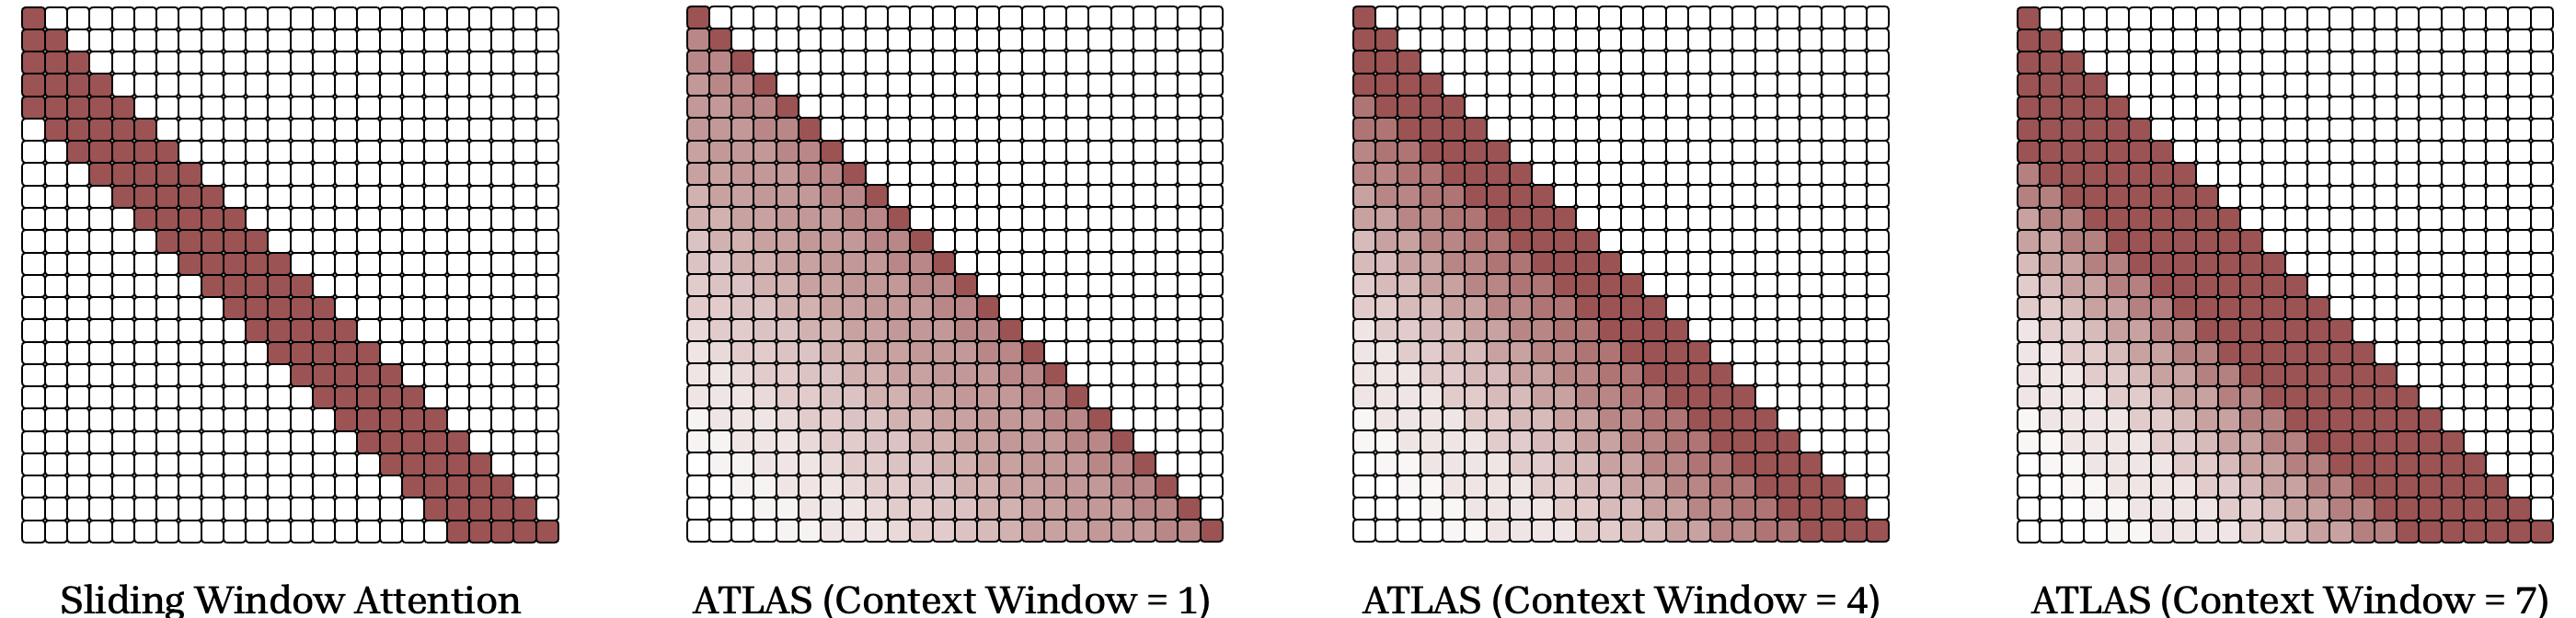
\includegraphics[width=0.9\linewidth]{Attn_ATLAS.png}
    \caption{The illustration of tokens dependencies in SWA and \model{} or \omodel{} with different context length.}
    \label{fig:attn_ATLAS}
\end{figure*}





\head{Beyond Gradient Descent} The concept of \learningrule{} rule and ``test time memorization of context'' can simply be extended to optimizing the objective in \autoref{eq:omega} with any arbitrary optimizer, even beyond simple gradient descent. We use two extreme cases for $c$ as the illustrations. In the first case, we let $c = 1$, $\gamma^{(t)}_i = 1$, and use gradient descent with momentum as the optimizers, resulting in the following update rule:
\begin{align}
    &\M_t = \alpha_t \M_{t-1} + \SSS_t \\
    &\SSS_t = \theta_t \SSS_{t-1} - \eta_t \nabla \ell(\M_{t-1}; \vk_t, \vv_t).
\end{align}
This update rule is equivalent to the long-term neural memory in Titans~\citep{behrouz2024titans}. In the second case, using a linear memory $\M$, letting $\gamma^{(t)}_i = 1$, and $c$ be equal to the context length, the memory update process is equivalent to optimizing the (regularized) least-squares problem:
\begin{align}
    \M_t = \min_{\M} \sum_{i = 1}^{t} \left\| \M \vk_i - \vv_i \right\|^2_2.
\end{align}
\citet{von2023uncovering} suggest directly optimizing the above objective and use Sherman-Morrison formula~\citep{sherman1950adjustment} to recursively calculate the inverse term in the optimal solution. Despite the optimality of memory, such direct solutions comes with the cost of non-parallelizable training and also are limited to only the linear matrix-valued memory setup. Furthermore, as discussed earlier, the global nature without any direct hard gating terms (i.e., $\gamma^{(t)}_i$s) can force the model to \emph{not} prune the context, damaging the performance in longer sequences. 




\subsection{Parallelizing \learningrule{} Rule}\label{sec:parallelization}
While \learningrule{} rule provides a more general and expressive formulation for the design of memory modules than Hebbian or Delta learning rules, its applicability to large-scale models relies on its efficiency in training. To this end, we discuss a fast parallelizable training algorithms that does not add any significant computational overhead with the online counterpart version (i.e., $c = 1$). A  naive implementation requires materializing \( c \) gradients \( \nabla \ell \in \mathbb{R}^{d_{\text{in}} \times d_{\text{in}}} \), which can result in a significantly higher memory footprint and I/O cost when \( d_{\text{in}} \) is large. Also, to fully utilize hardware accelerators such as TPUs and GPUs, it is important to tensorize computations and maximize the use of \texttt{matmul} operations. Motivated by recent work~\citep{behrouz2024titans, sun2024learning}, we propose a simple sliding window masking strategy that supports efficient parallel training while avoiding substantial memory overhead. Specifically, we partition the input sequence with length $L$ into chunks of size \( b  \geq 1 \), each of which is represented by $\mathbf{S}_i = \{ \vx_{(i-1)b+1}, \dots, \vx_{i b}\}$. Then for each chunk, we calculate the gradients with respect to the last state of the previous chunk. For the sake of clarity, we first assume \( \gamma^{(t)}_i =  \eta_t \) for all positions in the sequence. When the chunk size is \( b = 1 \), the update rule is:
\begin{align}
    \M_t = \alpha_t \M_{t-1} - \eta_t \sum_{i=t-c+1}^{t} \nabla \ell(\M_{t-1}; \vk_i, \vv_i),
\end{align}
where \( \M_t \) is the model state at step \( t \), \( \alpha_t \) and \( \eta_t \) are the weight decay and learning rate parameters respectively, and \( (\vk_i, \vv_i) \) denote the input pair at position \( i \). In practice, we strike a balance between the fully recurrent form and the fully parallel form by dividing the sequence into smaller chunks. Within each chunk (intra-chunk), we apply parallel computation, while across chunks (inter-chunk), we adopt a recurrent computation scheme. We now define \( t' = t - \operatorname{mod}(t, b) \). That is, for time steps \( t \) such that \( t' \leq t < t' + b \), the update rule within each chunk becomes:
\begin{align} \label{eq:omega_chunk_update_rule}
    &\M_t = \alpha_t ... \alpha_{t'} \M_{t'} - \sum^{t}_{n=t'} \frac{\alpha_t ... \alpha_{t'}}{\alpha_n ... \alpha_{t'}}\eta_n \undermath{G_t}{\sum^{n}_{i=n-c+1}\nabla \ell(\M_{t'}; \vk_i, \vv_i)}
\end{align}
In our implementation, for $G_t$, we follow the same gradient computation approach as described in Titans~\citep{behrouz2024titans} but additionally apply a sliding window mask \( M_s \) during the broadcasting operation (e.g., using \texttt{einsum}). When \( c = 1 \), the sliding window mask \( M_s \) reduces to the identity matrix. For \( c > 1 \), \( M_s \) is an identity matrix except that the \( c - 1 \) positions immediately preceding each diagonal entry are also set to 1. This allows gradient contributions from a window of size \( c \), enabling efficient computation without materializing all gradients inside the chunk.




\section{\protect \textsc{DeepTransformer}s: Transformers with Deep Memory}\label{sec:deeptransformers}
Recent studies have extensively discussed Transformer architectures through the lens of associative memory~\citep{wang2025test, sun2024learning, behrouz2025Miras}. Accordingly, it is natural to ask how our discussions of memory capacity as well as \learningrule{} rule can affect Transformers. In this section, we discuss how our formulation of \learningrule{} rule is connected to Transformers and their sliding window counterparts (i.e., SWA). We then further provide two extensions to Transformers, each of which is a strict generalization of Transformers.  


\subsection{Online and Local Context Optimization of Memory}

\head{Connection to Sliding Window Attention}
\texttt{Softmax} attention block can also be reformulated as a non-parametric  solution to the $\ell_2(\cdot)$ regression  with  Nadaraya-Watson estimators~\citep{zhang2022analysis, fan2018local}:
\begin{align}
    \M^* = \arg\min_{\M} \sum_{i = 1}^{L} \mathbf{s}(\vk_i, \vq) \|\vv_i - \M \|^2_2
    = \sum_{i = 1}^{L} \frac{\mathbf{s}(\vk_i, \vq)}{\sum_{j = 1}^{L} \mathbf{s}(\vk_j, \vq)} \vv_i,
\end{align}
where $L$ is the sequence length. While this formulation optimizes the memory $\M$ with respect to the entire sequence length, one can limit the optimization process to the past $c$ tokens, resulting in:
\begin{align}
    \M^* = \arg\min_{\M} \sum_{i = t - c + 1}^{t} \mathbf{s}(\vk_i, \vq_i) \|\vv_i - \M \|^2_2  = \sum_{i = t-c + 1}^{t} \frac{\mathbf{s}(\vk_i, \vq)}{\sum_{j = t - c + 1}^{t} \mathbf{s}(\vk_j, \vq)} \vv_i, 
\end{align}
which is equivalent to the sliding window attention (SWA). This connection provides an important insight on the difference of attention and recurrent models: Not only attention is a non-parametric solution (contrary to the parametric nature of recurrent models), it globally optimizes its internal objective (attentional bias), while most recent modern recurrent models are online learners~\citep{sun2024learning, yang2024gated, behrouz2025Miras, peng2025rwkv7}\footnote{Two of the exceptions are Titans~\citep{behrouz2024titans} and Mesa-layer~\citep{von2023uncovering}, where Mesa-layer optimizes the memory with respect to all past tokens (comes with the cost of slow training), and Titans optimizes the memory with respect to all past tokens but with an implicit decay term (i.e., the result of the momentum) for each past token, maintaining parallelizability.}
. Our formulations of sliding window RNN and \learningrule{} rule fill this gap by optimizing the memory with respect to a context window of past tokens based on parametric methods, effectively memorizing the context instead of individual tokens.


\head{Deep Linear Attention}
As a novel baseline, we present Deep (Gated) Linear Attention (DLA) that replaces a matrix-valued memory in (gated) linear attention~\citep{katharopoulos2020transformers, yang2024gatedattn} with a deep neural network (e.g., $k$-layer MLP). As discussed earlier in (\ref{eq:heb}), using dot product similarity as the internal attentional bias results in linear attention. Thus, leveraging recent deep memory modules \citep{sun2024learning, behrouz2024titans, behrouz2025Miras}, we optimize the memory using gradient descent with dot product attentional bias:
\begin{align}\label{eq:DLA}
    \M_t = \alpha_t \M_{t-1} -  \eta_t  \nabla \ell(\M_{t-1}; \phi(\vk_t), \vv_t),
\end{align}
where $\ell(\M_{t-1}; \phi(\vk_t), \vv_t) = \inner{\M_{t-1}(\phi(\vk_t))}{\vv_t}$ and $\phi(\cdot)$ is a polynomial kernel. The training of DLA can simply be parallelized using the hybrid of linear and non-linear chunk-wise training, the same as \citet{sun2024learning, behrouz2024titans} and our discussion in \autoref{sec:parallelization}.



\head{Sliding Window Linear Attention}
Building upon the above intuition and the connection of our formulation to SWA, we present Sliding Window Linear Attention (SWLA) block. Following the formulation of linear attention in associative memory perspective~\citep{behrouz2025Miras}, we use dot product similarity (i.e., $\ell(\M_t; \vk_i, \vv_i) = \inner{\M_t(\vk_i)}{\vv_i}$) as the attentional bias and optimize the loss function using gradient descent. For the sake of clarity, we use a linear memory here to derive the closed form:
\begin{align}
    \M_t = \alpha_t\M_{t-1} - \eta_t \nabla \sum_{i = t - c + 1}^{t} \ell(\M_{t-1}; \phi(\vk_i), \vv_i) = \M_{t-1} +  \sum_{i = t - c + 1}^{t} \gamma^{(t)}_i \vv_i \phi(\vk_i)^{\top}
\end{align}
In the online case ($c=1$) and $\phi(\cdot) = (\cdot)$, this recurrence is the same as linear attention~\citep{katharopoulos2020transformers}. 









\subsection{Memory Capacity and Exponential Kernels}\label{sec:deeptransformer-capacity}
We first recall the formulation of \texttt{softmax} attention in Transformers (i.e., \autoref{eq:attention}):
\begin{align}\label{eq:attention2}
    &\mathbf{y}_i = \frac{1}{{\sum_{\ell = 1}^{i} \exp\left( \mathbf{q}_i^{\top} \mathbf{k}_{\ell}/\sqrt{d_{\text{in}}}\right)}} \sum_{j = 1}^{i} \exp\left( \mathbf{q}_i^{\top} \mathbf{k}_j/\sqrt{d_{\text{in}}}\right) \mathbf{v}_j,
\end{align}
which its $\exp(\cdot)$ kernel is not separable and so cannot be written as a recurrence. Following the discussion in \citet{polysketchformer-kacham2024}, one can see $\exp(\cdot)$ kernel (compared to polynomial kernel $\phi_p(\cdot)$) as a feature map that maps the input into an infinite dimension. That is, we define: 
\begin{align}\label{eq:infi-map}
    \phi^{*}(x) = \begin{pmatrix}
    1 \\
    \frac{x}{\sqrt{1}} \\
    \frac{x^{\otimes 2}}{\sqrt{2!}} \\
    \frac{x^{\otimes 3}}{\sqrt{3!}} \\
    \vdots
    \end{pmatrix}, \qquad\qquad \phi_p(x) = 
    x^{\otimes p},
\end{align}
where $x^{\otimes p} = x \otimes x^{\otimes (p-1)}$ is a ``self-tensoring'' operator with Kronecker product~\citep{polysketchformer-kacham2024} and so:
\begin{align}
    \exp(\vq_t^{\top} \vk_t) = \phi^{*}(\vq_t)^{\top} \phi^{*}(\vk_t).
\end{align}
Based on the above kernel, we can reformulate the attention (see \autoref{eq:attention2}) as: (we remove $1/\sqrt{d_{\text{in}}}$ term for the sake of simplicity)
\begin{align}
    &\mathbf{y}_i = \frac{1}{{\sum_{\ell = 1}^{i} \exp\left( \mathbf{q}_i^{\top} \mathbf{k}_{\ell}/\sqrt{d_{\text{in}}}\right)}} \sum_{j = 1}^{i}  \mathbf{v}_j \phi^{*}(\mathbf{k}_j)^{\top} \phi^{*}(\mathbf{q}_i)  = \frac{1}{{\sum_{\ell = 1}^{i} \exp\left( \mathbf{q}_i^{\top} \mathbf{k}_{\ell}/\sqrt{d_{\text{in}}}\right)}} \left(\sum_{j = 1}^{i}  \phi^{*}(\mathbf{v}_j \mathbf{k}_j)^{\top}  \right) \phi^{*}(\mathbf{q}_i) = \M_i \phi^{*}(\mathbf{q}_i),
\end{align}

This formulation, provides another important insight on the differences of attention and (kernel) recurrent models: \texttt{Softmax} attention as an associative memory has an unbounded memory and so can better memorize larger context into its parameters. Building upon this insight, we present \textsc{DeepTransformers} by replacing polynomial kernel with $\phi^{*}(\cdot)$ kernel in Deep Linear Attention formulation (\autoref{eq:DLA}), resulting in unnormalized formulation of:
\begin{align}\label{eq:DeepTransformers}
    \M_t = \M_{t-1} - \nabla  \inner{\M_{t-1}(\phi^{*}(\vk_t))}{\vv_t}.
\end{align}
In the special case of linear memory, we can derive the closed form for the above formulation as:
\begin{align}
    \M_t = \M_{t-1} - \nabla  \inner{\M_{t-1}\phi^{*}(\vk_t)}{\vv_t} = \M_{t-1} + \vv_t \phi^{*}(\vk_t)^{\top}  = \sum_{i=1}^{t} \vv_i \phi^{*}(\vk_i)^{\top}  \quad \Rightarrow \quad \mathbf{y}_t = \M_t \phi^{*}(\vq_t) = \sum_{i = 1}^{t} \vv_i \exp(\vq_i^{\top} \vk_i ) ,
\end{align}
which matches the output of the unnormalized Transformers. Therefore, \textsc{DeepTransformers} are strict generalizations of Transformers with \texttt{softmax} attention~\citep{transformers}.

\subsection{Deep Omega Transformer (\protect \textsc{Dot}): Transformers with \learningrule{} learning rule} \label{sec:dot}
Our above formulation of \textsc{DeepTransformers} is based on the (\ref{eq:heb}), which is also used in original Transformers. However, as discussed earlier, using more powerful memory management and learning rules in associative memory modules can further enhance their performance. To this end, we extend the above formulation by replacing the Hebbian rule with our \learningrule{} learning rule, resulting in an unnormalized formulation of Deep Omega Transformers (\textsc{Dot}):
\begin{align}
     \M_t = \M_{t-1} - {\nabla \sum_{i = t - c + 1}^{t} \gamma^{(t)}_i \left\| \M\left(\phi^{*}(\vk_i)\right) - \vv_i \right\|^2_2}.
\end{align}
We now discuss special instances of \textsc{Dot} to provide further intuition on its generalized formulation. 

\head{Linear Memory} This setup results in the following unnormalized formulation:
\begin{align}
     &\M_t = \left( \mathbf{I} - \sum_{i = t-c+1}^{t} \gamma^{(t)}_i \phi^{*}(\vk_i)\phi^{*}(\vk_i)^{\top} \right)  \M_{t-1} - \sum_{i = t-c+1}^{t} \gamma^{(t)}_i \vv_i\phi^{*}(\vk_i)^{\top} \\ 
     \Rightarrow \:\:&\mathbf{y}_t = \M_t \phi^{*}(\vq_t) = \left( \mathbf{I} - \sum_{i = t-c+1}^{t} \gamma^{(t)}_i \phi^{*}(\vk_i)\phi^{*}(\vk_i)^{\top} \right)  \M_{t-1} \phi^{*}(\vq_t) \ - \sum_{i = t-c+1}^{t} \gamma^{(t)}_i \vv_i\exp(\vq_t^{\top}\vk_i). 
\end{align}
\head{Online Case with $c=1$} We now let $c = 1$:
\begin{align}
    &\M_t = \left( \mathbf{I} - \eta_t \phi^{*}(\vk_t)\phi^{*}(\vk_t)^{\top} \right)  \M_{t-1} - \eta_t \vv_t \phi^{*}(\vk_t)^{\top} \\ 
    \Rightarrow \:\: &\mathbf{y}_t = \M_t \phi^{*}(\vq_t) = \left( \mathbf{I} - \eta_t \phi^{*}(\vk_t)\exp(\vq_t^{\top}\vk_t) \right)  \M_{t-1} \ - \eta_t \vv_t\exp(\vq_t^{\top}\vk_t). 
\end{align}
The above (unnormalized) formulation can be seen as the generalization of Transformers with Delta Rule. Therefore, due to the unbounded memory, \textsc{Dot} not only appends the new keys and values (similar to original Transformers), but it also replaces the new value with its predicted value from the previous state. 


\section{\model: A Locally Optimal Memory with High Capacity} \label{sec:model}
Although the design of \learningrule{} rule allows the model to memorize the context instead of individual tokens and also the use of polynomial (or exponential) feature mapping increases memory capacity, the memory management (i.e., optimization of mappings between keys and values) is still limited to a simple gradient descent. This choice of optimizer can lead the model to a low-quality solution at a local optima, damaging the performance of the model in longer contexts. To overcome this issue, we suggest using Muon optimizer~\citep{jordan2024muon} (with weight decay) that not only approximates second-order information, but it also mostly leverages matrix multiplication and can be parallelized across the sequence. Accordingly, the use of Muon for optimizing the internal objective in \autoref{eq:omega}, results in the following update rule:
\begin{align}
     &\M_t = \alpha_t \M_{t-1} - \eta_t \: \texttt{NewtonShulz-$k$}(\mathcal{S}_t),\\
     &\mathcal{S}_t = \theta_t \SSS_{t-1} + \nabla \sum_{i = t - c + 1}^{t} \gamma^{(t)}_i \left\| \M\left(\phi^{*}(\vk_i)\right) - \vv_i \right\|^2_2,
\end{align}
where $c$ is the local context length and $k$ is the number steps for \texttt{NewtonShulz} operations. For the additional discussion on the algorithm and this operation we refer the reader to \citet{jordan2024muon}. Following the literature on Muon optimizer, we know that when $k \rightarrow \infty$, then  $\texttt{NewtonShulz-$k$}(\mathcal{S}_t)$ converges to the nearest semi-orthogonal matrix to the momentum term $\SSS_t$ and so approximate second-order information with a lower error. Therefore, interestingly, parameter $k$ can be considered as an internal test-time compute parameter in \model, where using more steps can potentially result in better memorization. 


\subsection{Parallel Training}
In this section, we discussed how the training process of \model{} can be parallelized. For the sake of clarity, we assume $c=1$. Generalizing the process to arbitrary value for $c$ follows the procedure in \autoref{sec:parallelization}. We use the same process as we discussed in \autoref{sec:parallelization} and so chunk the sequence and compute all the gradients with respect to the last state of the previous chunk. Accordingly, using the recurrence of \model{} with momentum but without , we have:
\begin{align}
    &\M_t = \alpha_t \M_{t-1} + \SSS_t \\
    &\SSS_t = \theta_t \SSS_{t-1} - \eta_t \nabla \ell(\M_{t'}; \vk_t, \vv_t).
\end{align}

Since $t'$ is the last state of the previous chunk, we can calculate all the gradients before hand and so we let $u_t = \nabla \ell(\M_{t'}; \vk_t, \vv_t)$. Therefore, we have:
\begin{align}
    &\M_t = \alpha_t \M_{t-1} + \SSS_t \\
    &\SSS_t = \theta_t \SSS_{t-1} - \eta_t u_t.
\end{align}
Now by expanding the second recurrence, we have:
\textbf{\begin{align}
    \SSS_t &= \theta_t \SSS_{t-1} - \eta_t \undermath{u_t}{\nabla \ell(\M_{t'}; \vk_t, \vv_t)}, \\
    \Rightarrow \SSS_t &= \undermath{\beta_t}{\theta_t ... \theta_1} \SSS_0 - \sum_{i = 1}^{t} \frac{\theta_t ... \theta_1}{\theta_i ... \theta_1} \eta_i u_i = \beta_t \SSS_0 - \Theta \odot E \odot G, 
\end{align}}
where $G$ is the gradient matrix, $E$ and $\Theta$ are diagonal matrices with value $\theta$ and $\eta$, and $\odot$ is broadcasting. 

The main advantage of the above formulation (chunk wise recurrence) is that the recurrence of momentum is independent of the state of memory. That is, we can calculate all the momentum terms in the beginning of the chunk using the above formulation. Now in the Muon case, we want to use Newton-Schulz algorithm on the momentum terms, which results in:
\begin{align}
    &\SSS'_t \leftarrow \texttt{Newton-Schulz5}(\SSS_t), \\
    &\M_t = \M_{t-1} + \SSS'_t.
\end{align}
Since the calculation of all $\SSS_t$s can be done in parallel, the calculation of $\texttt{Newton-Schulz5}(\cdot)$ can also be done in parallel. 














\head{Architectural Backbone}
As for the architectural backbone, we follow the recent modern recurrent models~\citep{behrouz2024titans, arora2024simple, yang2024parallelizing, Allen2025-canon} and use linear layers to project keys, values, and queries, followed by short convolution layers with size 4. We apply normalization on keys and queries to stabilize the training. We also follow \citet{behrouz2024titans} and use two hybrid variants of MAL and MAG for our \model{} model. The architectures are illustrated in \autoref{fig:arch-vis}. For models with deep memory architectures we use 2-layer MLP with residual connections:
\begin{align}
    \M(\cdot) = (\cdot) + W_1 \sigma(W_2 (\cdot)).
\end{align}
We further extend this memory architecture, which is commonly used in recent studies~\citep{behrouz2024titans, irie2021going, behrouz2025Miras}, to gated MLP layer as:
\begin{align}
    \M(\cdot) = (\cdot) + W_1 \left(\sigma\left(W_2 (\cdot)\right) \otimes W_3 (\cdot) \right),
\end{align}
where $W_1, W_2, W_3$ are linear learnable matrices. We refer to \model{} with the above memory architecture as \model++. 


\begin{figure*}
    \centering
    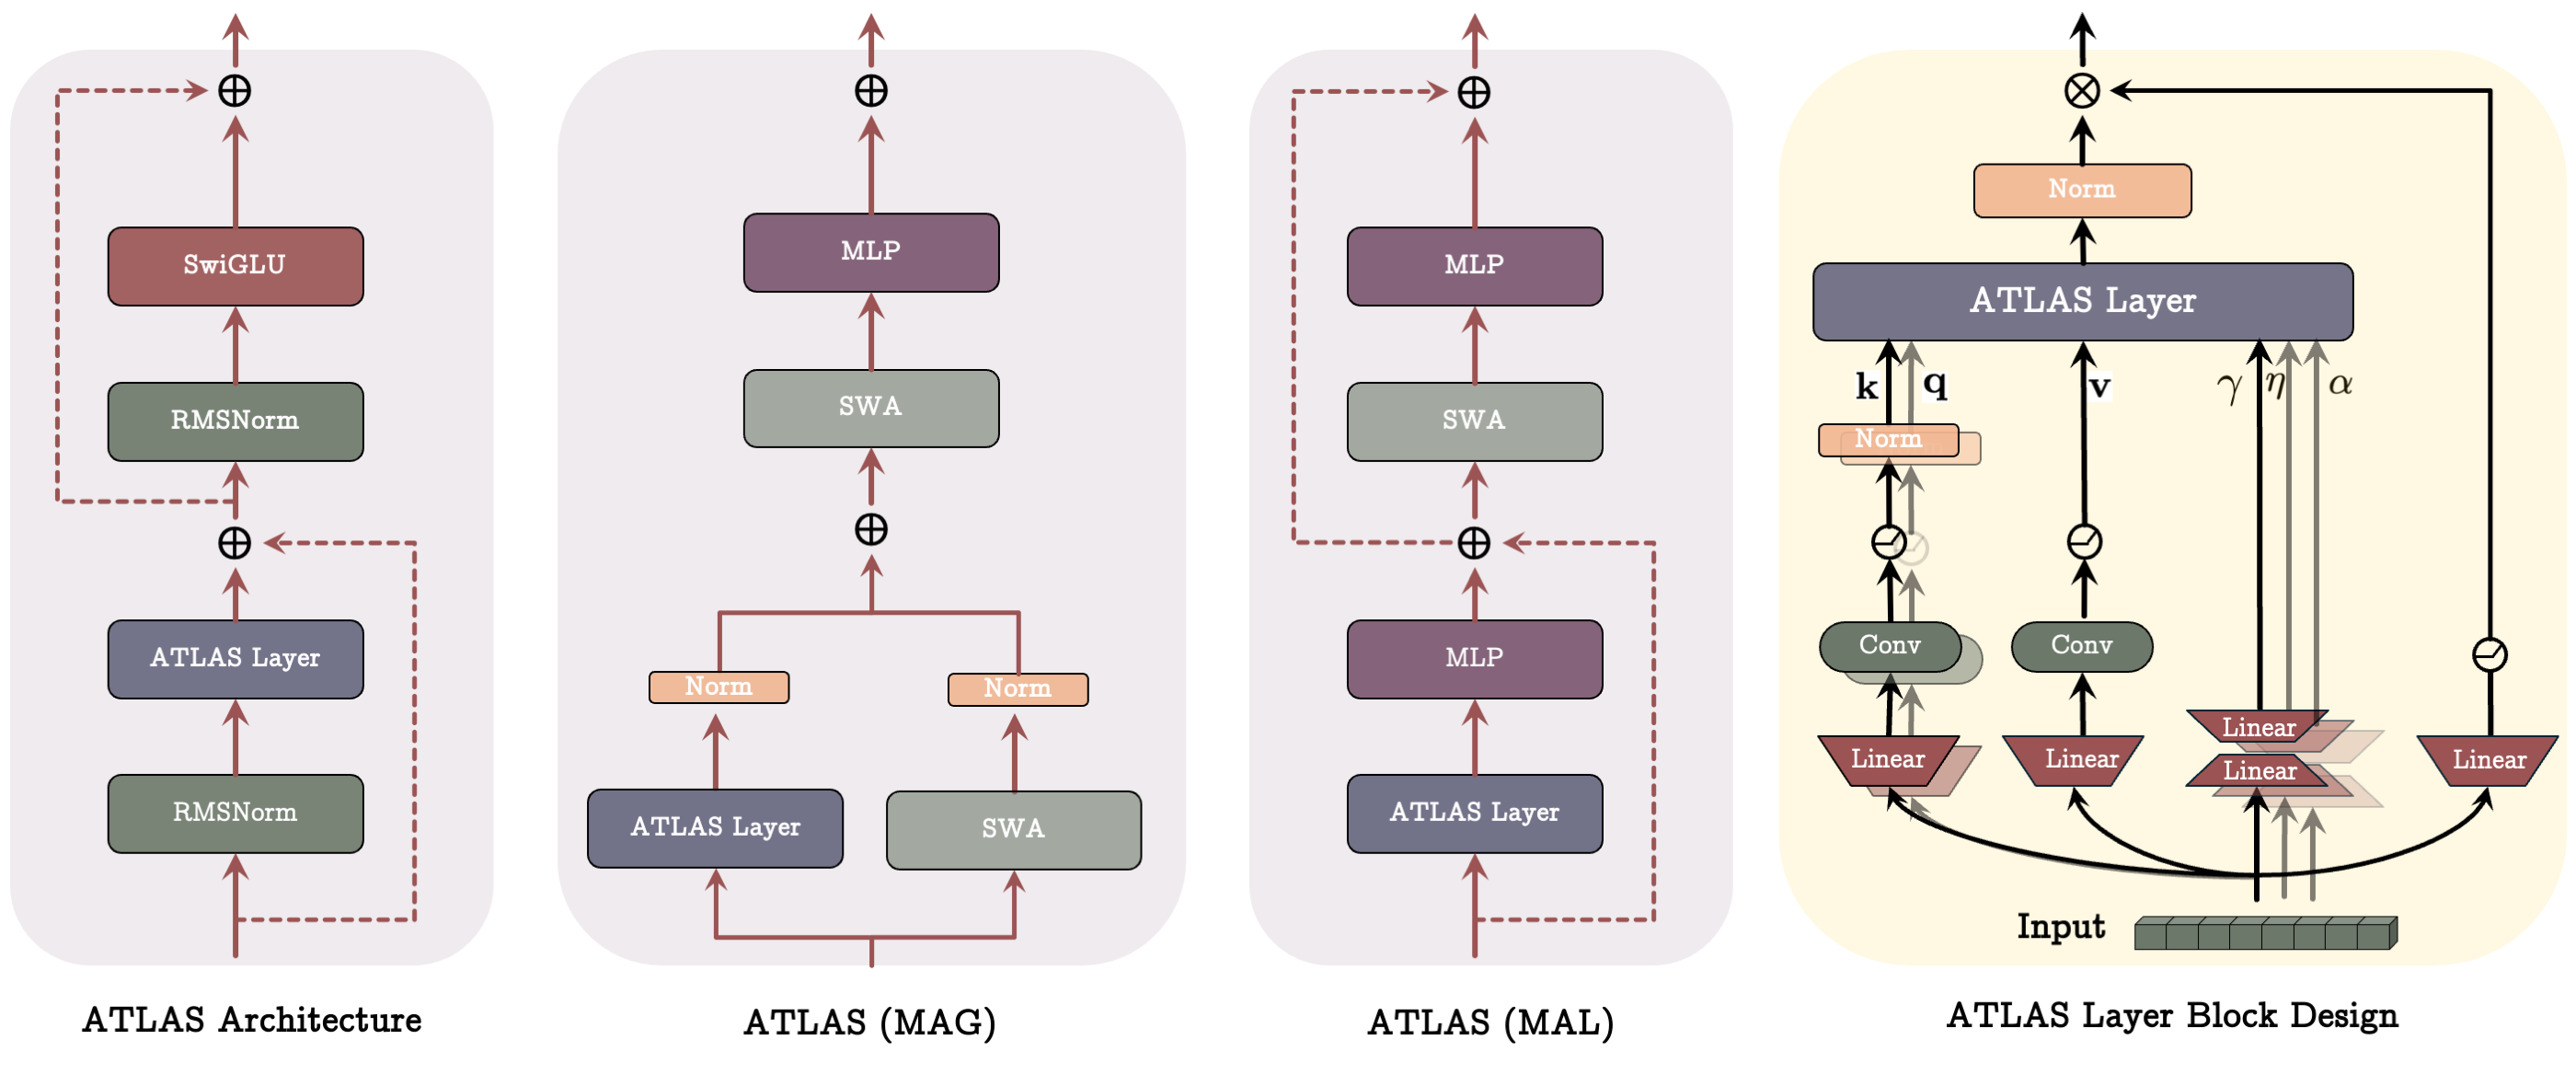
\includegraphics[width=0.9\linewidth]{Images/ATLAS.png}
    \caption{Visualization of the \model's (and our other variants') architecture, and its hybrid counterpart with SWA.}
    \label{fig:arch-vis}
\end{figure*}











































































